\section{Survey Design and Data}
\label{sec:survey}

\subsection{Telescope and calibrated measurements}
\label{sec:facility}

\SHARP\ uses the Xinglong 60/90~cm Schmidt telescope, with an effective
aperture of 0.60~m and an $f/3$ optical system. Its camera was developed at
the National Astronomical Observatories, Chinese Academy of Sciences.
The CCD has $9,216\times9,232$ pixels of $10~\mu$m, read through 16
simultaneous output channels. The typical scale is approximately
$1.15\asec$~pixel$^{-1}$, giving a nominal
$2.94^\circ\times2.95^\circ$ field of view. The observatory is listed under
Minor Planet Center (MPC) code 327. Table~\ref{tab:design} summarizes the
parameters used in the initial campaign.

The upstream reduction provides calibrated images (L1) and per-exposure
source catalogs (L2), following bias and flat-field correction, astrometric
solution, source extraction, and photometric calibration
\citep[in preparation]{Li2026InPrep}. Gaia EDR3 provides the astrometric
reference \citep{GaiaEDR32021,Lindegren2021EDR3}. Reference ICRS positions
at catalog epoch J2016.0 are propagated to the Julian year of the UTC
exposure start using the catalog proper motions and Astropy's
\texttt{apply\_space\_motion}, with the right-ascension proper motion
interpreted as $\mu_\alpha\cos\delta$. Parallax and radial velocity are
not supplied; sources with nonfinite propagated coordinates retain their
catalog positions. The propagated coordinates form the reference catalog
consumed by SCAMP, whose fitted TPV solution supplies the final image WCS. The moving-object analysis
begins from these products. The catalogs contain celestial and
image-plane coordinates, observing times, aperture magnitudes and their
uncertainties, and an image World Coordinate System (WCS). The source
measurements use fixed circular apertures in SExtractor
\citep{BertinArnouts1996}. Figure~\ref{fig:exposure} shows a representative image
and four cataloged asteroids.

The initial campaign uses white-light observations, denoted $W$ in the
observing records. The photometric reference is Gaia EDR3
\citep{GaiaEDR32021,Riello2021EDR3}. We retain the
existing notation \gaper\ for the calibrated L2 quantity
\texttt{Mag\_Aper4}: the fourth fixed aperture has a diameter of eight
pixels, or a radius of approximately $4.6\asec$. The symbol refers
throughout this paper to the calibrated white-light magnitude on the
reference scale defined below.

The photometric reference reader also computes propagated coordinates,
but the white-light calibration matches stars using their original
catalog coordinates. The calibration constructs a reference magnitude
from Gaia $G$ and the Gaia color $G_{\rm BP}-G_{\rm RP}$,
\begin{align}
x &= (G_{\rm BP}-G_{\rm RP})-0.340674898,\\
W_{\rm ref} &= G+0.1136777774 + P_W(x),\\
P_W(x) &= -0.03971196x^3+0.19464851x^2
          -0.11042587x-0.03542586.
\label{eq:color}
\end{align}
The per-exposure zero point $ZP$ is determined from an
18-pixel-diameter reference aperture. For a background-subtracted
eight-pixel aperture flux $f_8$ in ADU, the reported magnitude is
\begin{equation}
\gaper = ZP-2.5\log_{10}f_8+C_8,
\label{eq:apercal}
\end{equation}
where $C_8$ is the median difference between the instrumental
18-pixel and eight-pixel aperture magnitudes of the calibration stars.
The corresponding flux correction also scales the flux uncertainty.
This defines the adopted white-light scale; comparisons with predicted
asteroid $V$ magnitudes or standard passbands require color and response
information.

\begin{figure}[tbp]
\centering
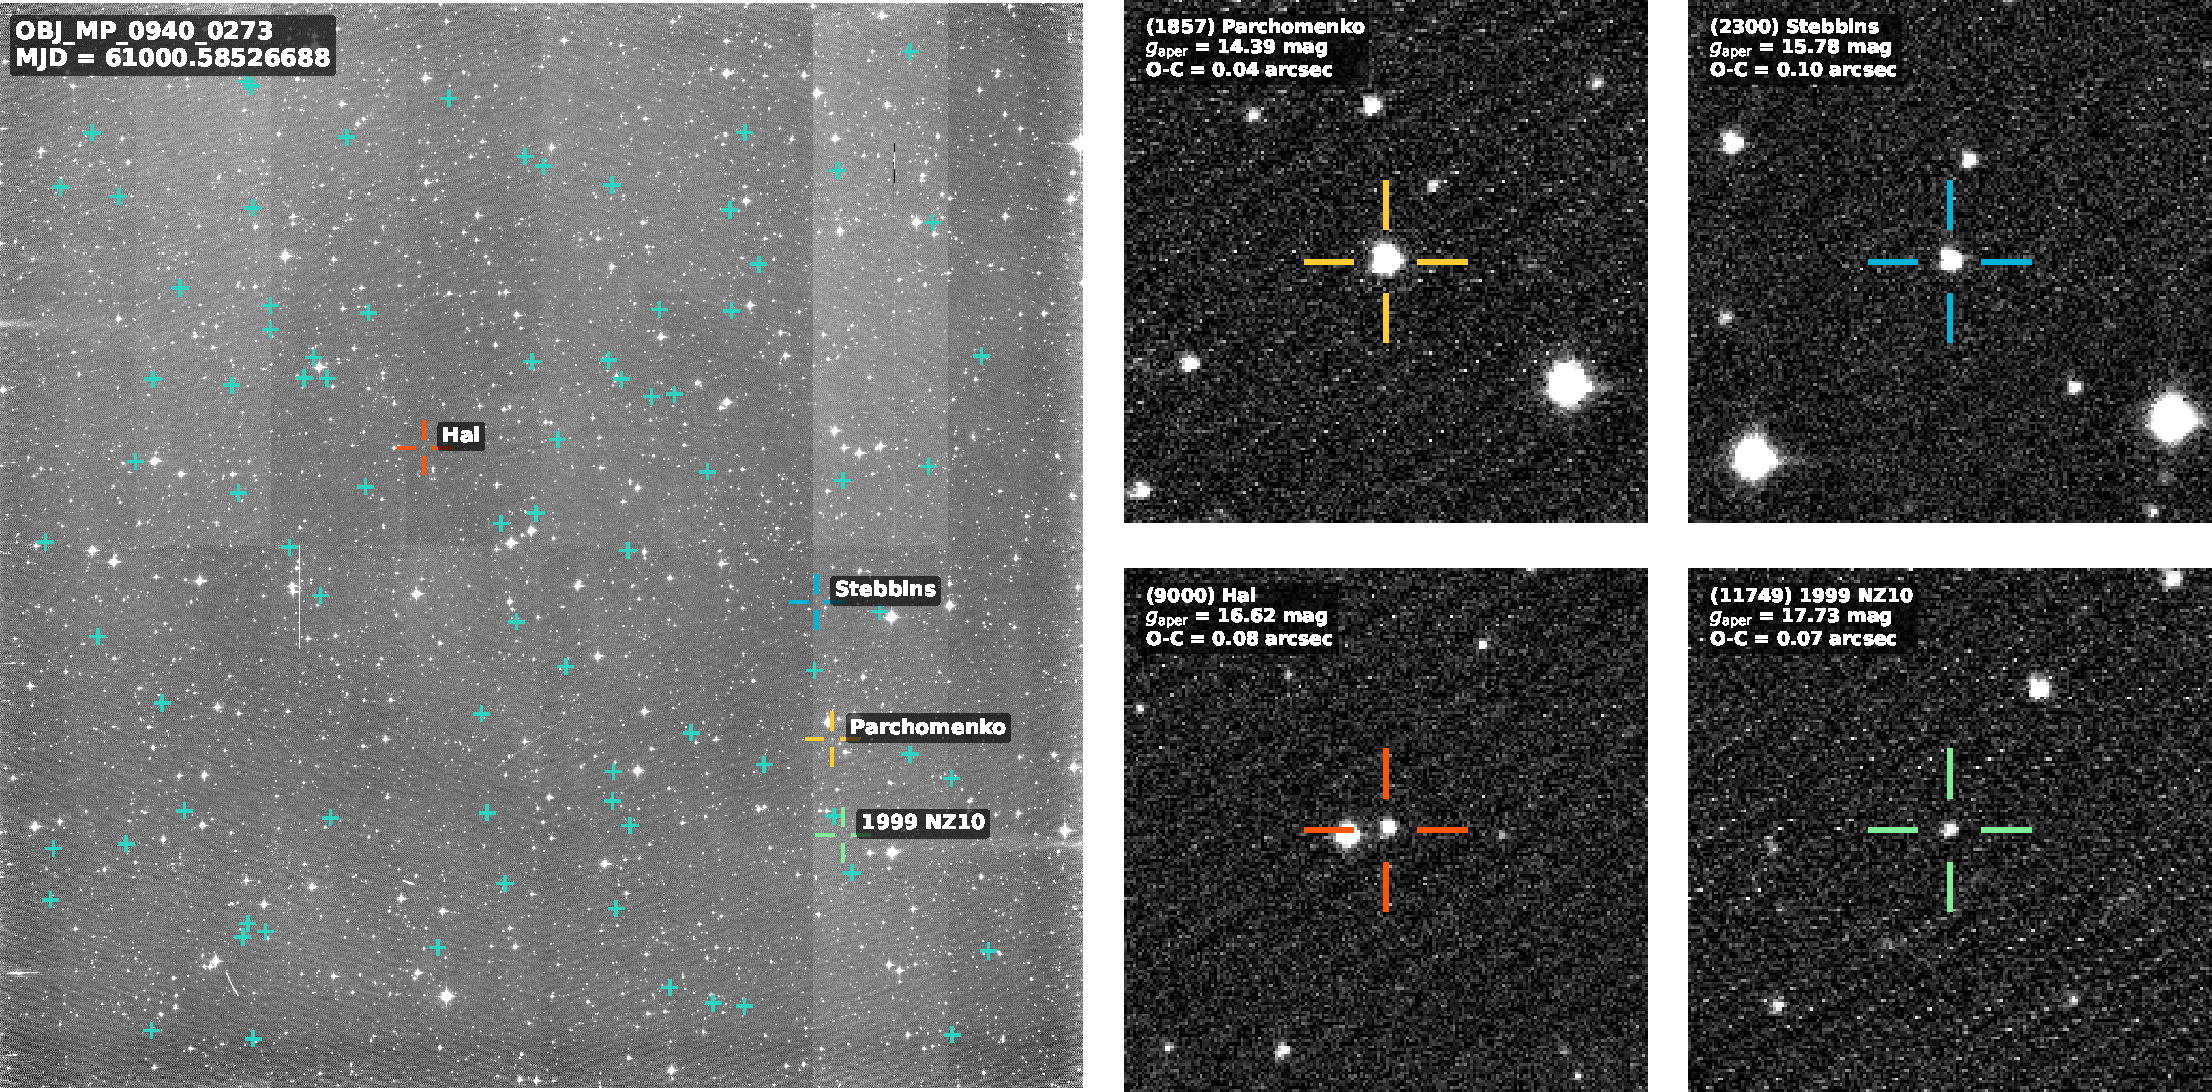
\includegraphics[width=0.98\linewidth]{fig01_exposure.pdf}
\caption{A representative 30~s white-light exposure obtained on 2025
November~21. The wide-field panel marks four known-asteroid associations,
and the four cutouts show their measured positions. Labels give the
calibrated white-light aperture magnitude \gaper\ and the radial
observed-minus-computed (O$-$C) separation within the $1\asec$ association
sample. The displayed MJD is the exposure start time; ephemeris matching
uses the exposure midpoint. The image uses a z-scale display with local
background treatment.}
\label{fig:exposure}
\end{figure}

\begin{table}[tbp]
\centering
\caption{Instrument and Initial Survey Parameters}
\label{tab:design}
\begin{tabular}{ll}
\toprule
Quantity & Value or convention\\
\midrule
Telescope & Xinglong 60/90~cm Schmidt, $f/3$\\
Detector size & $9,216\times9,232$ pixels\\
Pixel size / simultaneous readout channels & $10~\mu$m / 16\\
Typical pixel scale & $\simeq1.15\asec$~pixel$^{-1}$\\
Nominal field of view & $2.94^\circ\times2.95^\circ$\\
Observing band & $W$ (white light)\\
Reported aperture magnitude & Calibrated \texttt{Mag\_Aper4}, denoted \gaper\\
Measurement aperture & Eight-pixel diameter\\
Field library & 1,855 ecliptic fields\\
Standard exposure time & 30~s\\
Nominal visits and interval & Three visits; $\sim30$~min between starts\\
Readout allowance in scheduling & 15~s\\
Minimum planned target altitude & $30^\circ$\\
Known-asteroid prediction limit & $V<22.5$\\
Primary / auxiliary match radii & $1.0\asec$ / $1.5\asec$\\
Independent motion-search window & $3$--$63$~\rateunit\\
\bottomrule
\end{tabular}
\end{table}

\subsection{Observing strategy and analysis sample}
\label{sec:design}

The field library contains 1,855 pointings centered on an ecliptic band,
with field-center ecliptic latitudes from approximately $-18.5^\circ$ to
$+16.3^\circ$. The scheduling design selects observable fields according to
target altitude, seasonal visibility, Moon separation, and stored coverage
history, and groups nearby fields to limit slews. A normal sequence aims
for three visits, with a nominal 30~min interval between repeat starts.
The scheduler includes a 15~s readout allowance in addition to the nominal
30~s exposure and pointing overheads.

The observed footprint and cadence are measured from the actual WCS
pointings and exposure times in Section~\ref{sec:coverage}, encompassing
both completed and partial observing sequences.

\label{sec:cohorts}

The main archive covers 2025 November~15 through 2026 July~15. We select
unique physical exposures with calibrated catalogs, interpretable
exposure times, and usable WCS solutions consistent with the camera
geometry. Repeated files are counted once, and exposures with
inconsistent timing or astrometry are excluded. The selection retains
the range of seeing and photometric conditions in the usable archive;
the supplementary exposure ledger records the individual selections.

For the validated sample, we assign a physical observing night from the
exposure midpoint, with local noon in the Asia/Shanghai time zone as the
boundary. This avoids dividing an observing night at midnight and
resolves some differences from archive-directory labels. The resulting
sample contains 39,590 exposures on 129 physical nights, from 2025
November~16 through 2026 July~15. Its exposure, footprint, photometric,
and known-association statistics form the main performance results.

The linkage assessment compares stored moving-source links with known
identities, both in the original processing sample and after selecting
validated exposures and physical observing nights. The candidate sample
comes from the original image-review record; all 179 measurements in
its 58 retained links map to validated exposures. Their detailed results
are presented in Sections~\ref{sec:retention_results} and
\ref{sec:candidates}.

The scientific inputs and production methods considered in this paper
are restricted to material available by 2026 October~15. All quantitative
survey results refer to the November--July main archive. The archived
configuration and scientific inputs are identified in the data release.
